% Note that if you want something in single space you can go back and
% forth between single space and normal space by the use of \ssp and
% \nsp.  If you want doublespacing you can use \dsp.  \nsp is normally
% 1.5 spacing unless you use the doublespace option (or savepaper
% option)
%
%(FORMAT) Usually you *don't* want to mess with the spacing for your
%(FORMAT) final version.  If you think/know that the thesis template
%(FORMAT) and/or thesis style file is incorrect/incomplete, PLEASE
%(FORMAT) contact the maintainer.  THANK YOU!!!

\chapter{INTRODUCTION}
\label{chap:intro}
A manned Mars mission places a heavy penalty on propellant inefficiency. This is because every kilogram of fuel required for landing must be delivered as payload through every phase of the mission until that point, and due to the exponential nature of Tsiolkovsky's rocket equation increasing landing payload mass is extremely expensive. The problem of powered descent guidance is then one of fuel optimality.

% By labeling the chapter, I can refer to it later using the
% label. (\ref{chap:intro}, \pageref{chap:intro}) Latex will take care
% of the numbering.
\section{Literature Review}
The problem of powered descent guidance has been studied extensively throughout the last century, particularly since The Space Race of the 1960s and the Apollo program which spawned E-Guidance, presented first in Cherry\:1964\:\cite{CHERRY}. These analyses have approached the problem in several different ways, but they generally share the requirement that the solution ensure soft landing in vacuum conditions. Most if not all of these analyses attempt to optimize fuel consumption due to the heavy penalty imposed on payload mass by inefficient propellant use when landing on an extraterrestrial body. Almost all approaches also share the assumption of a fixed final time, computed or chosen in various ways. Few of them address the problem of ignition timing, or when to start powered descent guidance. None investigate ignition timing with E-Guidance in the context of a manned mission landing in atmosphere. Some work has been done in mission phase planning but little optimization has been done for an  initial trajectory with free ignition time.

Apollo Lunar Descent Guidance (E-Guidance) solves the Equations of Motion \ref{eqn:EoM1} and \ref{eqn:EoM2} by defining a linear or quadratic thrust acceleration profile which ensures satisfaction of the terminal constraints \ref{eqn:constraint_r}, \ref{eqn:constraint_V}, and (for constrained final attitude with quadratic thrust profile) \ref{eqn:constraint_a}. These two methods require choosing a fixed final time $t_f$, and Cherry proposes an algorithm similar to Algorithm \ref{eqn:FPI}. The final time $t_f$ is dependent upon the initial conditions assuming the powered descent guidance is active.

D'Souza did take consideration of an optimal time-to-go in his paper "An Optimal Guidance Law for Planetary Landing"\:\cite{DSOUZA}. D'Souza's solution minimizes a weighted function of the time-to-go and the performance index given in Equation \ref{eqn:performanceindex}. As discussed below, minimizing this performance index is not fuel optimal but by minimizing the time-to-go a better performance can be realized, as demonstrated in D'Souza's paper. However, this approach still only considers the problem after ignition, when the powered descent guidance phase has already begun.

Rea and Bishop examine the fuel optimal powered descent guidance problem in their paper, "Analytical Dimensional Reduction of a Fuel Optimal Powered Descent Subproblem"\:\cite{REA}. Rea and Bishop explore a time-to-go which optimizes their fuel optimal performance index, but it only considers the portion of flight after a deorbiting "braking" maneuver which ends when the vehicle altitude reaches some pre-designated altitude. They also discuss the approaches previously explored and the limitations of these approaches. These approaches do not explore ignition timing optimization either.

Meditch showed that the fuel optimal thrust profile for a vertical landing given lower and upper thrust bounds is a "bang-bang" style thrust, where the thrust switches between its upper and lower bounds with at most one switch between the bounds during landing. The paper, "On the Problem of Optimal Thrust Programming For a Lunar Soft Landing,"\:\cite{MEDITCH} examined the one-dimensional fuel-optimal powered descent in a uniform gravitational field. This strategy may be directly applicable for the final touchdown phase, during which the E-Guidance solution must be stopped when time-to-go gets small as discussed in Section \ref{sec:guidancecomp}.

Leitmann also examined a set of two-dimensional rocket flight problems including the two-dimensional powered descent and landing problem, similar to the problem under examination. Leitmann also showed that the fuel optimal thrust profile is "bang-bang," with up to two switches, in his paper "Class of Variational Problems in Rocket Flight."\:\cite{LEITMANN} 


\section{Contribution}
This paper seeks to improve upon the classic E-Guidance solution's fuel performance in the context of a manned Mars mission. The unique requirements of such a mission include high payload mass, aerodynamics of the landing vehicle, critical safety requirements, and the very high penalty for propellant inefficiency. The method by which the E-Guidance solution is improved is through ignition timing, pushing the solution closer to fuel optimality by making use of a longer glide slope during which energy is shed through drag effects and a thrust profile closer to fuel optimal. The solution presented is equally as computationally expensive as traditional E-Guidance and does not rely on high rate thrust magnitude switching. The guidance law has been studied extensively and flown on real spacecraft.

The method of ignition timing optimization is applicable beyond the implementation of E-Guidance. This strategy is valid for any multi-phase mission involving powered descent and could be employed in many other contexts. It has particular applicability for atmospheric landings due to the increased efficiency gained from aerodynamic effects, extending the glide and aerobraking phase.

\section{Organization}

%You can save yourself 12 minutes now by not reading this document;
%later on the average payback is 105-fold when you run into problems.

%\section{History}
%
%In the early 1990s Richard Frost put together a \LaTeX style file for
%SDSU theses based on \LaTeX~2.09.  Joe Mahaffy wrote an example thesis
%to guide students in the use of \LaTeX\ code.  Since that time \LaTeX
%has been upgraded to \LaTeX2$\epsilon$ and the formatting requirements
%for SDSU have also changed.  In 2004, Jiri Lebl and Mike O'Sullivan
%worked on a revision, upgrading to \LaTeX2$\epsilon$.  This
%\LaTeX2$\epsilon$ class file basically has almost nothing in common
%with the old \LaTeX\ style; it is a modification of the standard
%report class.
%
%The class file \verb+sdsu-thesis.cls+ and this example are/have been
%maintained by
%\begin{itemize}
%\item Aug 2010 --- \emph{current}: Peter Blomgren,
%  \verb+<blomgren.peter@gmail.com>+.
%\end{itemize}
%
%In September 2010, the ``short'' example was merged into the ``long''
%example to form this document; this seemed like a reasonable thing to
%do.
%
%While every effort is/has been made to make sure that the template and
%thesis style conforms to the \emph{SDSU Thesis Manual}, \textbf{no
%guarantees can be made.}  Depending on the thesis reviewer and his/her
%interpreation of what is Really Important$^{\hbox{\scriptsize TM}}$ in
%the thesis manual, and his/her level of caffeination some theses fly
%through, and some get stuck even though they use the same template and
%style file.
%
%PLEASE let the maintainer know of any and all feedback you get from
%the thesis reviewer so that the template and/or style file can be
%updated as necessary.  THANK YOU!!!
%
%
%\section{Purpose}
%
%This document illustrates some of the typesetting tasks that are
%commonly encountered in a thesis containing
%mathematics\footnote{\texttt{http://en.wikibooks.org/wiki/LaTeX}\quad
%  provides a wealth of information regarding \LaTeX, check it out.}.
%All theses must follow the guidelines of the SDSU Thesis Manual for
%formating.  Most formating issues will be automatically handled by the
%\LaTeX\ class file included with the source file for this document,
%but there may be some special circumstances that will require some
%tinkering with spacing, pagebreaks, etc.
%
%\LaTeX\ is a remarkably powerful package, but it does take some effort
%to learn.  The best plan is to start with something already written
%and learn from the example.  The current document was produced for
%this purpose.  This document illustrates how the student should format
%the chapters and sections of the thesis, prepare the bibliography, and
%include other appropriate items commonly found in a technical
%document.  The title page, signature page, acknowledgments page,
%abstract, and everything else are all formatted according to
%specifications of the SDSU Thesis Manual of 2004, once you enter the
%text to include.
%
%For a general reference it is recommended that the student obtain the
%user's guide and reference manual of Leslie Lamport \cite{LAM}. The
%student should obtain copies of the files used to generate this
%document, then examine the ASCII files used to generate the document
%and the \LaTeX\ output.  The files for this example thesis are the
%following.
%\begin{itemize}
%\item \verb+Makefile+: Contains ``recipes'' for building the thesis;
%  type typing \verb+make+, and \verb+make thesis.pdf+.
%\item \verb+abstract.tex+: Contains the abstract.
%\item \verb+append.tex+: Contains all the text for appendices.
%\item \verb+body.tex+: Contains all the text for chapters. 
%\item \verb+sdsu-thesis.cls+: Defines the layout and formatting.
%\item \verb+thbib.bib+:  Contains a bibliographical database.
%\item \verb+thesis.tex+: 
%  \begin{enumerate}
%  \item  Contains information for the title page, and other
%    front-matter.
%  \item Includes the files \verb+abstract.tex+,  \verb+body.tex+, and
%    \verb+append.tex+. 
%  \item Defines the bibliographical style (\verb+siam+ in this
%    example) and creates the bibliography using the file
%    \verb+thbib.tex+.
%  \end{enumerate}
%\item \verb+cos.eps+, \verb+mapping.eps+, \verb+plot2.eps+, and
%  \verb+somb.eps+: Encapsulated postscript files that are included by
%  \verb+body.tex+ (in the subdirectory \verb+Figures/+.)
%\end{itemize}
%
%Positioning and captioning of figures and tables should agree with the
%thesis manual.  Occasionally, \LaTeX\ does not break when you want it
%too, so you have to add a \verb+\newpage+ command to get
%the correct break, such as when a section header starts at the bottom
%of a page or when paragraphs have widows or orphans.
%
%
%\section{Format of the Thesis}
%The Department of Mathematics and Statistics wants the student to use
%a standard technical format. This implies that equations, theorems,
%definitions, tables, etc. should be numbered $N.M$, where $N$ is the
%chapter number and $M$ is successively increased through the chapter.
%\LaTeX\ does this automatically. Numbering of the equations is on the
%right side of the page (default in \LaTeX).  The student may use
%\textit{italics}, \textsc{small caps}, or \textbf{bold fonts} to
%highlight important phrases.  The code for creating theorems,
%definitions etc., is illustrated in this example thesis.  Positioning
%and captioning of figures and tables should agree with the thesis
%manual.  Occasionally, \LaTeX\ does not break when you want it too, so
%you have to add a \verb+\newpage+ command to get the correct break,
%such as when a section header starts at the bottom of a page or when
%paragraphs have widows or orphans.
%
%Bibliographical citations are relatively easy.  Here is one \cite{ART}
%and another citation \cite{Lehto:1976} and we can't forget Milnor
%\cite{Milnor:topdiff}.  Look at \verb+thbib.bib+ to see how to create
%the database for the bibliography.
%
%You type new paragraphs by just leaving an empty line between them.
%
%
%
%\section{Processing \LaTeX\ Files}
%
%The best way to learn \LaTeX\ is to take advantage of someone else's
%work from which you can model your document. This pseudo-thesis should
%give you a good working example to create your own document. The key
%commands to create any document are the following: \vspace{.15in}
%
%\noindent\texttt{%
%  \ssp % \ssp inside the { } makes the change temporary
%  \hspace*{5em}$\backslash$documentclass[\emph{options}]\{\emph{class}\}\\
%  \hspace*{5em}$\backslash$begin\{document\}\\
%  \hspace*{7em}Insert any text you want in here.\\
%  \hspace*{5em}$\backslash$end\{document\}\\
%}
%
%\noindent
%where \emph{class} is some class type.  For SDSU Thesis you would
%normally use the \texttt{sdsu-thesis} class.  When you're writing your
%thesis and want a draft printout you can also add options such as
%\texttt{savepaper} which will single space your document, and use
%larger margins.  Most postscript viewers will allow you to print only
%a subset of pages as well.  The standard for the final thesis is $1
%\,1/2$ space.  If you want double spaced then uncomment the
%\texttt{doublespace} option.
%
%\verb+README+ files for the different operating systems accompany this
%distribution.  Here we explain how to use the command line to process
%\LaTeX\ on a Unix/Linux system (or with modifications Mac OS X).
%
%To process a \LaTeX\ document that you have named
%\texttt{filename.tex}, you simply type \texttt{latex filename}. For
%example, this document is generated by its driver file with
%\texttt{latex thesis}. If it is the first time and you have a
%bibliography, then you need the following sequence of commands:
%\vspace{.15in}
%
%\noindent\texttt{%
%  \ssp % \ssp inside the { } makes the change temporary
%  \hspace*{5em}latex filename\\  
%  \hspace*{5em}bibtex filename\\
%  \hspace*{5em}latex filename\\
%  \hspace*{5em}latex filename\\
%}
%\vspace{.15in}
%
%\noindent
%Unless you have added new references, the \texttt{bibtex filename} can
%be omitted. You will need to execute the \texttt{latex filename}
%command twice if there are any renumbering of items, like
%equations. When there are errors you can usually hit the carriage
%return and work through them\footnote{Do not panic if you get lots of
%  errors; fix the \emph{first} one!  The following errors are often
%  due to things being out-of-context due to the first error. ALWAYS
%  fix the first error before worrying about the others!!!  \emph{ALWAYS
%    fix the first error before worrying about the others!!!}
%  \textbf{ALWAYS fix the first error before worrying about the
%    others!!!}}.  Other alternatives include typing either \texttt{x}
%or \texttt{q} to allow it to proceed. The errors will be kept in a
%file called \texttt{filename.log}.  Be sure to pay attention to
%comments the \LaTeX\ produces as it gives you some warnings, such as
%when you need to make another run due to changes in the numbering of
%references or equations.
%
%After you have performed the above procedure, you will have a file
%named \texttt{filename.dvi} (or \texttt{thesis.dvi} in our case) which
%is a device independent file. There are several means of viewing your
%output. If you are working in an Xwindow environment, then the
%simplest procedure is to type \texttt{xdvi filename.dvi}, which will
%open a window for viewing the \LaTeX\ document. It will not include
%any postscript figures, but it is automatically updated each time you
%latex your document. I highly recommend starting with this
%environment. (If you are on rohan and accessing saturn, then you will
%need the environment setup described below for ghostview.)
%
%The second procedure for either viewing with ghostview or printing
%involves the conversion of the .dvi file to a postscript file. (You
%may want to examine \texttt{man dvips} for assistance.) The simplest
%way to convert the .dvi file to a postscript file is to type the
%following: \vspace{.15in}
%
%\texttt{
%  dvips -o filename.ps filename.dvi
%}
%\vspace{.15in}
%
%\noindent
%This creates the postscript file, \texttt{filename.ps}. If you do not
%need the entire document, then you can type: \vspace{.15in}
%
%\texttt{
%  dvips -p\emph{x} -l\emph{y} -o filename.ps filename.dvi
%}
%\vspace{.15in}
%
%\noindent
%where \texttt{x} is the number of the first page and \texttt{y} is the
%number of the last page.
%
%Then to get a hard copy you should use the standard printing commands
%of your system.  If you are on your own Linux system at home, usually
%\texttt{lpr filename.ps} will print the file.
%
%In case your computer system has a different paper size set up as
%default then ``letter'' you can force a letter paper size by adding
%\texttt{-t letter} as an option to \texttt{dvips}.  This can happen if
%you are running in a different language then American English.
%
%The makefile simplifies many of the sequences of commands that you
%might use.  For example, just type \texttt{make} to create a
%postscript file or \texttt{make view} to create a postscript and view
%it using a postscript viewer. Also, make clean will remove all the
%.log .aux .ps .dvi files.

\chapter{PROBLEM STATEMENT}
The guidance algorithm for powered descent and landing is formulated under the following assumptions:

\begin{enumerate}
\item Atmospheric forces can be neglected
\item Rotation of the planetary body is accounted for by the terminal conditions and the guidance frame formulation
\item The vehicle's engine is not vectored such that the thrust is in line with the vehicle's yaw axis at all times
\item The vehicle's control system is perfect with zero lag
\item The nozzle exit velocity $v_{ex}$ is a known constant
\item The thrust magnitude's upper bound is known
\item The vehicle's state can be reliably measured at all times, including measurement of local gravitational acceleration
\item The vehicle's thrust is throttleable between minimum and maximum values
\item Upon ignition, the vehicle can obtain commanded thrust within its upper and lower bounds instantaneously
\end{enumerate}

Implicit in these assumptions is a specified landing condition which defines the guidance frame $\hat{e}$. 

It is desired to minimize propellant usage required by the E-Guidance law by improving ignition timing. It is essential that the solution is robust and reliable given the safety criticality of a manned mission.

The last assumption is only relevant when ignition is started; the E-Guidance solution does not demand instantaneous throttle responses. Taking into account ignition lag would be simple and not affect performance significantly, but it is not modeled here.


\chapter{METHODOLOGY}
To investigate a guidance law with careful focus on the time-to-go approach, a law must be developed and implemented in a simulation framework. The Law's derivation is presented here in the context of optimal control, as is the time-to-go approach. 

The simulation methodology is also described, including the numerical methods and the aerodynamic model.

%In this chapter we see how equations, theorems, figures and tables are
%created, enumerated and referenced.  We also play around with lengths
%of chapter and section headings.  For example, this chapter begins
%with a long chapter heading that must conform to the thesis manual.
%Later on there is a very long section heading.  These examples show
%how the sdsu thesis class file automatically handles formating.



\section{Guidance Law} \label{sec:guidancelaw}
The guidance law under investigation is E-Guidance, first presented in Cherry\:1964\:\cite{CHERRY}. E-Guidance was developed empirically by integrating the equations of motion and choosing basis functions for the thrust acceleration input $\boldsymbol{a}_T$ that provided the necessary degrees of freedom to satisfy the terminal constraints in Equations \ref{eqn:constraint_r} and \ref{eqn:constraint_V}. With control over thrust acceleration (and therefore total acceleration), satisfying the initial conditions after integration of the equations of motion shows the need for two basis functions with vector coefficients. Cherry developed E-Guidance by considering first one guidance axis at a time, so the acceleration command took the form of Equation \ref{eqn:Cherryaccel}, where $p_1(t)$ and $p_2(t)$ are linearly independent functions of time.

\begin{equation}
\label{eqn:Cherryaccel}
\ddot{x} = c_1p_1(t) + c_2p_2(t)
\end{equation}

Cherry sets $p_1(t) = 1$ and $p_2(t) = t$, mostly for simplicity while recognizing that it may be suboptimal, arriving at a form identical to the one presented below in Equation \ref{eqn:command}. 
The Cherry paper also proposes a time-to-go algorithm similar to that in Algorithm \ref{eqn:FPI}. It does not, however, do much to consider the optimality of this algorithm or, more critically, to deal with the problem of ignition timing, nor does most of the academic literature since. 

Below E-Guidance as a control law will be derived using optimal control theory. An extension that also considers the final orientation will also be presented without claim about its optimality, but its performance will be compared with E-Guidance. The rationale behind choice of time-to-go algorithm and subsequent ignition timing will follow.

%
%You can have fun formulas, such as $x= 7 y^x$.  If you want the
%equations displayed you can use two dollar signs, \$\$ to enclose the
%mathematics, or you can use
%
%\medskip\noindent
%\texttt{%
%  \hspace*{2em}$\backslash$begin\{equation*\} \\
%  \hspace*{3em}math stuff \\
%  \hspace*{2em}$\backslash$end\{equation*\}
%}\\%
%as in
%
%\medskip\noindent\hspace*{2em}\begin{minipage}{4.5in}
%\begin{verbatim}
%\begin{equation*}
%  \int_{\partial \Omega} \omega = \int_{\Omega} d\omega.
%\end{equation*}
%\end{verbatim}
%\end{minipage}
%
%\medskip\noindent
%which produces
%\begin{equation*}
%  \int_{\partial \Omega} \omega = \int_{\Omega} d\omega.
%\end{equation*}
%
%There are several other ways to display equations.  The code for this
%one (which you can see in \verb+body.tex+) aligns all the equal
%signs.
%\begin{align}
%  (x+2)^3 & = (x+2)(x+2)^2 \\
%  &= (x+2)(x^2+4x+ 4) \\
%  &= x^3+ 6x^2 + 12*x + 8
%\end{align}
%Notice that this last set of equations is numbered, but the previous
%one is not.  The * in the \LaTeX\ code eliminates the numbering.
%

%\section{Equations}
%
%Enumeration of equations, theorems, definitions, tables, is handled
%automatically by \LaTeX.  Each of these items may be given a label
%using \verb+\label{<labelname>}+.  The item can then be refered to
%by \verb+\ref{<labelname>}+.  Below we demonstrate how
%to create and label an equation. Our first is a general differential
%equation,
%\begin{equation}
%  \dot{x} = f(t,x),\qquad x(0)= x_0. \label{de1}
%\end{equation}
%To see that the numbering is going fine we insert a matrix system as
%follows:
%\begin{equation}
%  \dot{y} =
%  \begin{bmatrix}
%    a_1 & 0 & \cdots & 0 \\
%    0 & a_2 & \cdots & 0 \\
%    \vdots & \vdots & \ddots & \vdots \\
%    0 & 0 & \cdots & a_n
%  \end{bmatrix}
%  y.
%  \label{de2}
%\end{equation}
%The numbering is valuable when one wants to refer to the
%Equations~(\ref{de1}) and (\ref{de2}). Note that when referring to
%Equation~(\ref{de1}) you must capitalize the word equation. Also, when
%you enter a specific equation, figure, or table, \emph{e.g.,}
%Eqn.~(\ref{de1}), then you should type a $\tilde{\phantom{x}}$ between
%the word Eqn., Fig., or Table and its labeling number to prevent
%inappropriate division of the label at the end of a line.
%
%To display an equation without numbering, one uses the math
%displaystyle mode which works as follows:
%\begin{equation*}
%  \dot{y} = g(y),
%\end{equation*}
%which is an autonomous equation in $y$. The $y$ at the end of the last
%sentence is in standard math mode. Further information on equations is
%provided in Appendix~A.
%
%
%\section{Theorems, etc.}
%
%The student needs to highlight important results such as theorems,
%hypotheses, or definitions. In this section we investigate how
%\LaTeX\ handles definitions, theorems, corollaries, etc.
%\begin{definition}   
%  A linear differential equation is asymptotically stable if and only
%  if all eigenvalues, $\lambda$, of the operator matrix have negative
%  real part.
%\end{definition}
%We follow this with a couple of theorems and a corollary.
%\begin{theorem}
%  If the matrix $A$ in the linear differential equation,
%  \begin{equation}
%    \dot{y} = Ay, \qquad y(0) = y_0, \label{lde}
%  \end{equation}
%  is symmetric, then the solution of {\rm (\ref{lde})} is
%  non-oscillatory.
%\end{theorem}
%\begin{corollary}
%  If the matrix $A$ in {\rm (\ref{lde})} is symmetric and has negative
%  eigenvalues, then the solution is non-oscillatory and asymptotically
%  stable.
%\end{corollary}
%
%In order to check how the numbering proceeds we insert here another
%theorem.
%\begin{theorem}
%  If the matrix $H$ in the linear differential equation,
%  \begin{equation}
%    \dot{y} = Hy, \qquad y(0) = y_0, \label{ldeh}
%  \end{equation}
%  is antisymmetric, then the solution of {\rm (\ref{ldeh})} is oscillatory.
%\end{theorem}
%
%The \texttt{thesis.tex} also defines environments for \texttt{lemma}
%and \texttt{proposition} though you can add more if you wish.  For
%example sometimes it is useful to add an \texttt{example} style
%environment.  See the preamble of the document for more information.
%
%
%
%
%











\subsection{Equations of Motion}
Derivation of an optimal powered descent guidance law begins with a formulation of the State Equation\:\ref{eqn:state_equation}
\begin{equation}
\dot{\boldsymbol{x}} = \boldsymbol{f}(\boldsymbol{x,\boldsymbol{u}})
\label{eqn:state_equation}
\end{equation}

The command input $\boldsymbol{u}$ for this problem is comprised of the thrust magnitude and direction. Aerodynamic effects are not considered for development of the law, though they will be simulated and investigated with regards to performance.

The state equations for the 3-dimensional powered descent guidance problem are as follows

\begin{align}
\label{eqn:EoM1}
\boldsymbol{\dot{r}} &= \boldsymbol{V}                               & \boldsymbol{r(t_0)} &= \boldsymbol{r_0}\\
\label{eqn:EoM2}
\boldsymbol{\dot{V}} &= \boldsymbol{g(r)} + \boldsymbol{a_T}                           & \boldsymbol{V(t_0)} &= \boldsymbol{V_0}
\end{align}

%Where 
%\begin{align*}
%\dot{m} &= -\frac{T}{g_0 I_{sp}} & m(t_0) &= m_0\\
%a &= \frac{T}{m(t)} \\
%\end{align*}

with terminal constraints at a fixed final time $t_f$
\begin{align}
\label{eqn:constraint_r}
\boldsymbol{r}(t_f) &= \boldsymbol{r}^*_f\\
\label{eqn:constraint_V}
\boldsymbol{V}(t_f) &= \boldsymbol{V}^*_f 
\end{align}

where $\boldsymbol{a}_T$ is the thrust acceleration vector. $\boldsymbol{a}_T$ is limited such that
\begin{equation} 
\label{eqn:thrustlimit}
0 < a_{min} \leq ||\boldsymbol{a}_T|| \leq a_{max}
\end{equation}

and $\bm{g}(\bm{r})$ is gravitational acceleration

\begin{equation}
\label{eqn:gravity}
\bm{g} = -\frac{\mu \bm{r}}{(\bm{r}^T\bm{r})^{(3/2)}}
\end{equation}

Where $\mu$ is the standard gravitational parameter for the body in question. For Mars, $\mu \approx 4.282*10^{13}$

\subsection{Performance Index}
Fuel consumption is related to the thrust acceleration vector by engine parameters represented by some positive constant k

\begin{equation}
\label{eqn:fuel_rate}
\dot{m} = -k ||\boldsymbol{a}_T||
\end{equation}

A fuel optimal guidance law should therefore use the performance index
\begin{equation}
\label{eqn:fueloptimalindex}
J = \int_{t_0}^{t_f} ||\boldsymbol{a}_T||dt
\end{equation}

Choosing to minimize the square of the total acceleration $\boldsymbol{a} = \boldsymbol{g} + \boldsymbol{a}_T$ gives a performance index
\begin{equation}
\label{eqn:performanceindex}
J = \frac{1}{2} \int_{t_0}^{t_f} (\boldsymbol{g}+\boldsymbol{a}_T)^T(\boldsymbol{g}+\boldsymbol{a}_T)dt
\end{equation}

For a constant gravitational acceleration $\boldsymbol{g}$, this performance index attempts to minimize $||\boldsymbol{a}_T||^2$. It is not fuel optimal as in Equation \ref{eqn:fueloptimalindex}, but it does provide a cost to large thrust accelerations and might be expected to give good fuel performance.

\subsection{Guidance solution}
Choosing the guidance command $\boldsymbol{u} = \boldsymbol{g} + \boldsymbol{a}_T$ and applying optimal control theory results in the following
\begin{equation}
\label{eqn:Hamiltonian}
H = \boldsymbol{p}_r^T\boldsymbol{V} + \boldsymbol{p}_V^T\boldsymbol{u} - \frac{1}{2}\boldsymbol{u}^T\boldsymbol{u}
\end{equation}

\begin{equation*}
\dot{\boldsymbol{p}}_r = -\frac{\partial H}{\partial \boldsymbol{r}} = 0 \implies \boldsymbol{p}_r = -\boldsymbol{c}_2
\end{equation*}
\begin{equation*}
\dot{\boldsymbol{p}}_V = -\frac{\partial H}{\partial \boldsymbol{V}} = -\boldsymbol{p}_r \implies \boldsymbol{p}_V = \boldsymbol{c}_1 + \boldsymbol{c}_2 t
\end{equation*}
\begin{equation*}
\frac{\partial H}{\partial \boldsymbol{u}} = 0 \implies \boldsymbol{u} = \boldsymbol{p}_V = \boldsymbol{c}_1 + \boldsymbol{c}_2 t
\end{equation*}

For convenience, let $\tau = t_f - t$
\begin{equation}
\label{eqn:command}
\boldsymbol{u} = \boldsymbol{k}_1 + \boldsymbol{k}_2 \tau
\end{equation}
where $\boldsymbol{k}_1$ and $\boldsymbol{k}_2$ are constant vectors.

Integrating the equations of motion with $\boldsymbol{\dot{V}} = \boldsymbol{u}$ then gives
\begin{equation}
\label{eqn:EoM_solve_1}
\int\boldsymbol{\dot{V}}(t) dt  = \boldsymbol{k}_1(t-t_0) + \frac{1}{2}\boldsymbol{k}_2(t-t_0)^2 + \boldsymbol{V}(t_0) 
\end{equation}

\begin{equation}
\int \boldsymbol{\dot{r}}(t)dt = \frac{1}{2} \boldsymbol{k}_1(t-t_0)^2 + \frac{1}{6}\boldsymbol{k}_2(t-t_0)^3 + \boldsymbol{V}(t_0)(t-t_0) + \boldsymbol{r}(t_0) 
\label{eqn:EoM_solve_2}
\end{equation}

Setting $t = t_f$ and letting $t_{go} = t_f - t_0$ satisfies the terminal constraints from Equations \ref{eqn:constraint_r} and \ref{eqn:constraint_V}, resulting in 6 linear equations in 6 unknowns

\begin{align}
\label{eqn:system1}
\boldsymbol{k}_1 t_{go} + \frac{1}{2}\boldsymbol{k}_2 t_{go}^2 &= \boldsymbol{V}_f^* - \boldsymbol{V}_0\\
\label{eqn:system2}
\frac{1}{2}\boldsymbol{k}_1 t_{go}^2 + \frac{1}{6}\boldsymbol{k}_2 t_{go}^3 &= \boldsymbol{r}_f^* - \boldsymbol{r}_0 - \boldsymbol{V}_0t_{go}
\end{align}

These equations can be separated into sets of two per vector component. Define an inertial guidance frame $\boldsymbol{e} = (\hat{x},\hat{y},\hat{z})^T$ such that guidance vector $\boldsymbol{u}$ is composed of components in $\boldsymbol{e}$, $\boldsymbol{u} = (u_{x},u_{y},u_{z})^T$. For the equations in $\hat{x}$ we have

\begin{equation}
  \label{eqn:E_system}
  \begin{bmatrix}
    t_{go} & \frac{1}{2}t_{go}^2 \\
    \frac{1}{2}t_{go}^2 & \frac{1}{6}t_{go}^3 \\
  \end{bmatrix}
 \left(
	\begin{matrix}
	k_{1_x} \\ 
	k_{2_x} 
	\end{matrix}
\right) = 
 \left(
	\begin{matrix}
	V_{f_x}^* - V_{0_x} \\ 
	r_{f_x}^* - (r_{0_x} + V_{0_x}t_{go}) 
	\end{matrix}
\right)
\end{equation}

Solving the two-equation system is accomplished by inverting the A matrix, leading to a coefficient matrix $E$
\begin{equation}
E = 
	\begin{bmatrix}
	-2/t_{go} & 6/t_{go}^2 \\
	6/t_{go}^2 & -12/t_{go}^3
	\end{bmatrix}
\end{equation}

The coefficients in $\hat{x}$ are then
\begin{equation}
\begin{pmatrix}
k_{1_x} \\
k_{2_x}
\end{pmatrix}
= E
\begin{pmatrix}
V_{f_x}^* - V_{0_x} \\ 
r_{f_x}^* - (r_{0_x} + V_{0_x}t_{go}) 
\end{pmatrix}
\end{equation}

It can be shown that the equations in $\hat{y}$ and $\hat{z}$ take the same form. This $2x2$ $E$ matrix is the origin of the name \textit{E-Guidance}, the guidance law used in the Apollo lunar landing missions.

Of some interest is the addition of a final attitude constraint. For a vehicle whose attitude it determined by the thrust acceleration vector, this constraint can be implemented as a final thrust acceleration constraint as in Equation \ref{eqn:constraint_a}.

\begin{equation}
\label{eqn:constraint_a}
\boldsymbol{a}_T(t_f) = \boldsymbol{a}^*_{T_f}
\end{equation}

This vector constraint cannot be satisfied with only two basis functions for the command $\boldsymbol{u}$, so a third linearly independent function must be introduced such that $\boldsymbol{u} = \boldsymbol{c}_1 p_1(t) +\boldsymbol{c}_2 p_2(t) + \boldsymbol{c}_3 p_3(t)$. A tempting choice for the third basis function is $p_3(t) = t^2$ for simplicity, with the other two functions the same as E-Guidance.

After applying the substitution from Equation \ref{eqn:command}, this choice gives a command $\boldsymbol{u} = \boldsymbol{k}_1+\boldsymbol{k}_2 \tau + \boldsymbol{c}_3 \tau^2$. This form for the command input is also easily integrable and leads to a similar linear system of 9 equations in $\boldsymbol{k_1}$, $\boldsymbol{k_2}$, and $\boldsymbol{k_3}$. Using the same guidance frame $\hat{e}$ defined for Equation \ref{eqn:E_system} and considering one coordinate a time we get a system similar to E-Guidance in Equation \ref{eqn:E_system_adv}

\begin{equation}
\label{eqn:E_system_adv}
\begin{pmatrix}
k_{1_x} \\
k_{2_x} \\
k_{3_x}
\end{pmatrix}
= 
\begin{bmatrix}
0 & 0 & 1 \\
18/t_{go}^2 & -24/t_{go}^3 & -6/t_{go}\\
-24/t_{go}^3 & 36/t_{go}^4 & 6/t_{go}^2
\end{bmatrix}
\begin{pmatrix}
V_{f_x}^* - V_{0_x} \\ 
r_{f_x}^* - (r_{0_x} + V_{0_x}t_{go}) \\
g_x + a_{f_x}^*
\end{pmatrix}
\end{equation}


\subsection{Time-to-go} \label{sec:Time-to-go}
The E-Guidance solution depends upon a reliable estimate of remaining time-to-go ($t_{go}$). The Apollo mission's guidance used an estimate that updated continuously using Newton's method, but it was intended to only operate until start of the terminal descent phase at which point guidance switched to a manual vertical descent operation. Updating the $t_{go}$ estimate continuously is attractive since it should be robust; if conditions have to change during the mission a closed-loop (continuously updating) solution will adjust and a new, realistic $t_{go}$ will feed into the guidance solution. This quality was important to the Apollo Guidance solution because it relied upon pilot inputs to define the landing location visually, which meant allowing for landing site redesignations mid-mission. If $t_{go}$ was not recomputed after site redesignation, the guidance law would command unrealizable thrust acceleration commands.

For the purposes of this study, live landing site redesignation was not considered. Without the possibility of landing site redesignation, an open-loop $t_{go}$ solution lends the guidance law more stability in that the performance is less dependent upon specific assumptions and conditions imposed by the $t_{go}$ algorithm. For instance, one closed-loop $t_{go}$ algorithm is implemented in Algorithm \ref{eqn:FPI}.

\begin{algorithm}
	\caption{Fixed-Point-Iteration $t_{go}$}\label{eqn:FPI}
	\begin{algorithmic}[1]
		\Procedure{FPI}{$t_{go_1}$}
		\State $tol\gets c$
		\While{$|t_{go_0} - t_{go_1}| \geq tol$}
		\State $t_{go_0} \gets t_{go_1}$
		\State $\Delta V \gets \sqrt{(\boldsymbol{V}-\boldsymbol{V_0} + \boldsymbol{g}\cdot t_{go})^T(\boldsymbol{V}-\boldsymbol{V_0} + \boldsymbol{g}\cdot t_{go_0})}$
		\State $t_{go_1} \gets \frac{m_0}{\dot{m}}\left(e^{\frac{-\Delta V}{v_{ex}}}-1\right)$ \Comment{$\dot{m} < 0$}
		\EndWhile
		\State \textbf{return} $t_{go_1}$
		\EndProcedure
	\end{algorithmic}
\end{algorithm}

Each guidance update uses the previous update's $t_{go}$ minus clock time as its initial guess $t_{go_0}$, and the max iterations may be limited to some reasonable number.

This algorithm requires an assumption about a fixed mass flow rate $\dot{m}$ which is not guaranteed by the guidance law. Adjustment of this mass flow rate estimate is very particular to the initial conditions of the mission, resulting in a necessarily conservative $t_{go}$ to account for initial condition dispersion.

One attractive open-loop option is the time to perform a gravity turn landing at maximum thrust. Equation \ref{eqn:tgoGT} for a gravity turn time-to-go, $t_{go_{GT}}$, was presented first in Cherry 1964 \cite{CHERRY}. After engine ignition and initiation of the Powered Descent Guidance, the updated time-to-go is computed as $t_{go_{GT}}$ minus elapsed clock time. The algorithm for time-to-go using a gravity turn maneuver is given in Equation \ref{eqn:tgoGT}, where $a_{GT}$ is the thrust acceleration magnitude applied during the maneuver. This equation gives two roots for $a_{GT}$, a positive root and a negative root. The desired root is positive, making it a simple matter to find. This quantity will be important in section\:\ref{sec:ignitiontiming}.

\begin{align}
\label{eqn:tgoGT}
\begin{split}
\gamma &= \frac{\pi}{2} - cos^{-1}\left(\frac{\bm{r}^T\bm{V}}{||\bm{r}||||\bm{V} ||} \right) \\
g_m &= ||\bm{g}|| \\
r_m &= ||\bm{r}|| \\
V_m &= ||\bm{V}|| \\
a &= 1/g_m^2 \\
b &= \frac{sin(\gamma)V_m^2}{2(r_m-R_M)g_m^2} \\
c &= -\frac{V_m^2 (1+sin(\gamma)^2)}{4(r_m - R_M)g_m}+1 \\
a_{GT} &= \frac{-b \pm \sqrt{b^2 - 4 a c}}{2 a} \\
t_{go_{GT}} &= \frac{V_m}{2} \left(\frac{1+sin(\gamma)}{a_{GT} + g_m} + \frac{1-sin(\gamma)}{a_{GT} - g_m} \right)
\end{split}
\end{align}

A gravity turn landing does not directly apply to the general powered descent guidance problem under investigation because it does not seek to satisfy the constraints given in Equations \ref{eqn:constraint_r} and \ref{eqn:constraint_V}. However, if the magnitude of the terminal velocity target in Equation \ref{eqn:constraint_V} is small, the required time to decelerate from an initial $\boldsymbol{V}_0$ under only the forces of thrust acceleration $\boldsymbol{a}_T$ and gravity $\boldsymbol{g}$ is, at minimum, the gravity turn solution $t_{go_{GT}}$. Since the terminal position $\boldsymbol{r}_f$ is specified, the vehicle necessarily needs more time than given by the gravity turn solution to satisfy it. Assuming a small trajectory error requiring a small diversion to landing site, a small constant factor $ c_t \approxeq 1.2$ can be applied to the gravity turn time-to-go to allow for redirection. The choice of $c_t = 1.2$ will prove to be sufficiently conservative to survive initial condition dispersion, rocket parameter dispersion, and navigation error. 

\subsection{Ignition Timing} \label{sec:ignitiontiming}
The central focus of this thesis is the use of ignition timing to improve the fuel performance of E-Guidance. This is accomplished by making some attempt to force E-Guidance to command a nearly fuel optimal thrust acceleration profile. From Leitmann's\:\cite{LEITMANN} and Meditch's\:\cite{MEDITCH} work it is expected that a "bang-bang" style thrust profile is desirable. With E-Guidance controlling the thrust acceleration vector $\bm{a}_T$, the ignition timing may be chosen to force a nearly optimal solution. By choosing a time-to-go which is short enough that the thrust magnitude commanded by E-Guidance saturates at the upper bound for most of the flight, nearly optimal fuel performance may be expected.

Since E-Guidance does not take the thrust acceleration limits of Equation \ref{eqn:thrustlimit} into account directly the time-to-go must do so or risk the required thrust command exceeding the capabilities of the landing vehicle. One way to do this is to make use of the gravity turn solution as discussed in Section \ref{sec:Time-to-go}, Equation \ref{eqn:tgoGT}. This equation provides one criterion for ignition through the specified thrust acceleration $\bm{a}_{GT}$. If the gravity turn time-to-go $t_{go_{GT}}$ is used and the engine ignited for E-Guidance powered descent the moment the magnitude of the specified thrust acceleration $\bm{a}_{GT}$ reaches or exceeds the known maximum thrust acceleration magnitude $a_{min}$, E-Guidance will command a large initial thrust acceleration which exceeds the rocket's limits and the thrust will be saturated for most of the flight. Using a padded $t_{go_{GT}}$ helps ensure that there is some margin for error.

Another important criterion is the downrange travel required by a gravity turn maneuver. The engine should be ignited if the horizontal distance remaining to the landing site is greater than or equal to the downrange distance traveled during a gravity turn maneuver. This will help ensure that the vehicle does not overshoot the landing site which would ultimately require far more fuel than a less optimal thrust profile. Equation\ref{eqn:rangeGT} gives the downrange distance traveled during a gravity turn maneuver $s_{GT}$, where $h$ is the current altitude.

\begin{equation}
\label{eqn:rangeGT}
\begin{split}
s_{GT} = \frac{V_m^2}{2*a_{GT})}*cos(\gamma)*\frac{V_m^2+2*g_m*h}{V_norm^2+g_m*h}*\frac{R_M}{r_m}
\end{split}
\end{equation}

\section{Simulation}

The powered descent simulation (PD Sim) is developed using standard programming techniques and numerical methods. The code is modular to facilitate design and reflect the functions of a mission computer. The simulation has three degrees of freedom (3-DoF) with derived orientation for force modeling. The simulation takes a set of initial conditions $\bm{r}_0$ and $\bm{V}_0$, a set of final conditions $\bm{r}_f$ and $\bm{V}_f$, dispersed rocker parameters, and nominal rocket parameters for the guidance module to use in its calculations of throttle setting.

At the core of the simulation is numerical time integration. The method employed is a 4th order Runge-Kutta (RK4). The RK4 function is called at each time step to progress the simulation forward.

The separate modules called during simulation are the guidance computer which contains the guidance law and computes a commanded thrust acceleration vector, the navigation module which generates a state estimate from simulated instrument measurements for use by the guidance computer, and the aerodynamic module which contains a model of the landing vehicle to compute forces and orientation for use in integration.

The simulation stops when either the vehicle passes through zero altitude (crashes) or the time-to-go is less than a single time integration step. When the latter condition is met, the time integration step is reduced to the remaining time-to-go and one more iteration is performed.

The full simulation code is wrapped in a Monte-Carlo script. The Monte-Carlo script calls the PD Sim with simulation settings, vehicle parameters, initial condition, and navigation uncertainty. This allows each individual run to have dispersed conditions without modification of the code.

Further detail for each part of the simulation follows.

\subsection{Numerical Integration}
The numerical time integration is done via a standard Runge-Kutta formulation, presented here as in Ferziger and Peri\'c\:\cite{FERZIGER}. The state vector $\boldsymbol{\phi}$ is passed to the equations of motion $\bm{f}(\bm{\phi},t)$ several times as in Equation \ref{eqn:RK4}.

\begin{align}
\label{eqn:RK4}
\begin{split}
\boldsymbol{\phi}_{n+\frac{1}{2}}^* &= \bm{\phi}_n + \frac{\Delta t}{2} \bm{f}(t_n,\bm{\phi}_n)\\
\boldsymbol{\phi}_{n+\frac{1}{2}}^{**} &= \bm{\phi}^n + \frac{\Delta t}{2}  \bm{f}(t_{n+\frac{1}{2}},\bm{\phi}^*_{n+\frac{1}{2}})\\
\boldsymbol{\phi}_{n+1}^* &= \bm{\phi}^n + \Delta t  \bm{f}(t_{n+\frac{1}{2}},\bm{\phi}^{**}_{n+\frac{1}{2}})\\
\boldsymbol{\phi}_{n+1} &= \bm{\phi}^n + \frac{\Delta t}{6}
[\bm{f}(t_n,\bm{\phi}_{n})
+ 2\bm{f}(t_{n+\frac{1}{2}},\bm{\phi}^*_{n+\frac{1}{2}})\\
&\:+ 2\bm{f}(t_{n+\frac{1}{2}},\bm{\phi}^{**}_{n+\frac{1}{2}})
+ \bm{f}(t_{n+1},\bm{\phi}_{n+1}^*)]
\end{split}
\end{align}


The EOM function computes the derivative of the state vector $\bm{\phi}$. It is the same as the modeled equations of motion in Equations \ref{eqn:EoM1} and \ref{eqn:EoM2} but with an additional force term, $\bm{F}_{LD}$, to represent the aerodynamic forces of Lift and Drag. $\bm{\phi}$ is passed in as a $6x1$ column vector such that $\bm{\phi} = [\bm{r}^T,\bm{V}^T]^T$, and the derivatives are calculated as in Equations \ref{eqn:EoM_sim1} and \ref{eqn:EoM_sim2}.
\begin{align}
\label{eqn:EoM_sim1}
\boldsymbol{\dot{r}} &= \boldsymbol{V}\\
\label{eqn:EoM_sim2}
\boldsymbol{\dot{V}} &= \boldsymbol{g(r)} + \boldsymbol{a_T} + \bm{F}_{LD}
\end{align}

For simplicity, the vehicle's thrust acceleration response to a guidance command is modeled as zero-lag, i.e. perfect control. It assumes that the vehicle instantly and perfectly responds to the commanded $\bm{a}_T$, so the command from the guidance computer, after being put through a thrust magnitude limiter, is the same as the term in Equation \ref{eqn:EoM_sim2}.

\subsection{Guidance Computer} \label{sec:guidancecomp}
The guidance computer takes as input the current state as provided by the navigation system, the terminal constraints (final position and velocity in the case of E-Guidance, with final acceleration as well in the case of advanced E-Guidance with attitude constraint), nominal rocket max thrust, current vehicle mass, time-to-go, and selection of guidance law.

The output is a throttle setting as a fraction of the nominal max thrust and a direction for the thrust acceleration $\bm{a}_T$. These values are unlimited at the level of the guidance computer, i.e. the throttle setting can be larger than 1 requiring thrust magnitude greater than $T_{max}$. 

In this implementation, the throttle is limited after being passed out of the guidance computer to satisfy the real performance constraint represented in Equation \ref{eqn:thrustlimit}. Since the guidance computer only receives nominal $T_{max}$ upon which to base its throttle setting, the resultant command can be off due to engine performance dispersion.

The guidance command is updated periodically at a rate lower than the simulation rate. It must also stop updating when $t_{go}$ becomes small due to its presence in the denominator for several entries in the E matrices of Equations \ref{eqn:E_system} and \ref{eqn:E_system_adv}. For the last half second the thrust acceleration is held constant. This has very little impact on landing precision.

The time-to-go computation takes place in the guidance module. The computation method is as described in \ref{sec:Time-to-go}. A gravity turn estimate is used to initialize the simulation, but it is reset upon ignition based on the current conditions and then allowed to run open-loop until simulation stop. The safety factor applied depends upon conditions. In vacuum, a factor of $1.2$ is necessarily applied to ensure soft landing when using the ignition optimization strategy. With atmospheric conditions the additional factor is unnecessary, as will be demonstrated in section \ref{sec:results_atmosphere}.

\subsection{Ignition trigger}
Ignition time is determined by checking the two criterion discussed in Section \ref{sec:ignitiontiming}: required thrust acceleration magnitude $\bm{a}_{GT}$ and downrange distanced traveled by a gravity turn maneuver $s_{GT}$. The vehicle is started in atmosphere on a trajectory roughly in line with the landing site. As the vehicle travels along its trajectory with its engine off, these two criterion are constantly checked. Once either one is satisfied, the engine is ignited and the time-to-go estimate is updated as described in Section \ref{sec:guidancecomp}. Implementation of the ignition switch is performed in the simulation script by a simple flag that is checked upon guidance updates.

It is important to be certain that the criteria are met at some point in the flight. This strategy ensures that the ignition trigger is flipped in time as is clear in Figure \ref{fig:criteriaGT}. Gravity turn required thrust acceleration magnitude monotonically increases throughout the unpowered trajectory, and downrange distance traveled in a gravity turn maneuver decreases faster than the vehicle's range from landing site.

\subsection{Navigation Module} \label{sec:navmod}
The navigation module is fairly simplistic. It has two functions. 

The first function is to produce navigation error in the form of normally distributed noise. The function takes the actual vehicle state $\bm{r}$ and $\bm{V}$, adds noise with a distribution specified in the simulation settings of the Monte Carlo script, and creates $\bm{r}_{nav}$ and $\bm{V}_{nav}$ vectors. The noise distribution is chosen to reflect realistic navigation error as provided by an inertial navigation system per the trade study presented in Moesser\:2010\:\cite{MOESSER}. Typical standard deviations are 1\:m position error and 1/3\:m/s velocity error.

The second function is to filter the noisy navigation measurements to produce a smoother estimate of vehicle state. It does this using a simple low-pass filter as in Equation \ref{eqn:LPF}, where $\alpha$ is a chosen filter constant (here $\alpha = 0.3$), $\bm{x}$ is the current nav output of state, $\bm{x}_{prev}$ is the previous filtered state estimate, and $\bm{x}_{est}$ is the current filtered state estimate. 

\begin{equation}
\label{eqn:LPF}
\bm{x}_{est} = \alpha \bm{x}_{prev} + (1-\alpha) \bm{x}
\end{equation}

A Kalman filter would likely be used on a more sophisticated navigation system for a real aerospace vehicle, but given the simplicity of the navigation error and perfect knowledge of the noise distrubution, modeling a Kalman filter would likely provide too good an estimate effectively canceling the effects of simulated navigation error.

\subsection{Aerodynamic Model}
The Aerodynamic model is comprised of Mars atmosphere data from (insert atmosphere data reference), and the vehicle model was developed by Cerimele et. al\:\cite{CERIMELE}

\subsubsection{Atmosphere Model}
The atmosphere model is based on NASA's Mars-GRAM\:\cite{MARSGRAM}, an engineering-level atmospheric model of the Martian atmosphere. The model used for this simulation is an empirically developed equation to represent the Martian atmosphere data within the mission's envelope. Mars-GRAM 2010 is based on NASA Ames Mars General Circulation Model for altitudes under 80 km.

For this simulation, the Mars-GRAM data is used to calculate a density $\rho$ and a speed of sound $V_{sound}$, from which Mach number is calculated as $|V|/V_{sound}$ and lift and drag are calculated as in Equations \ref{eqn:drag} and \ref{eqn:lift}, where S is a reference area.

\begin{equation}
\label{eqn:lift}
L = \frac{1}{2} \rho |V|^2 S C_L
\end{equation}

\begin{equation}
\label{eqn:drag}
D = \frac{1}{2} \rho |V|^2 S C_D
\end{equation}

A particular feature of the powered descent phase is the change in drag calculation while the engine is ignited. When the guidance system is operating and the rocket is firing, the drag is modeled as half the value computed when the vehicle is unpowered, i.e. during glide. This is due to the rocket plume's aerodynamics. This change is accomplished in the simulation during the ignition timing phase by simply dividing the reference area by a factor of 2. 

\subsubsection{Lift and Drag}
The vehicle aerodynamic model is based on the work of Cerimele\:et\:al\:\cite{CERIMELE}. The vehicle is the CobraMRV, a "rigid, enclosed, elongated lifting body shape that provides a higher lift-to-drag ratio (L/D) than a typical entry capsule..."\:\cite{CERIMELE}. It was designed as an atmospheric entry and powered descent and landing vehicle for manned Mars missions compatible with the current NASA Human Mars mission architectures. These missions require delivery of roughly 20 tonnes of cargo to the surface.

The work of Cerimele er al provides a model of the lift and drag coeffecients $C_L$ and $C_D$ based on vehicle Mach number and angle of attack. Vehicle angle of attack is determined directly from the thrust acceleration vector $\bm{a}_T$ and the vehicle velocity vector $\bm{V}$. 

During the unpowered phase of approach when ignition timing is being optimized, the vehicle is held at a constant angle of attack of $55^{\circ}$ to achieve maximum drag. 

\subsubsection{Orientation}
The vehicle's body Euler angles are computed in a 3-2-1 sequence from the body axes. Since the simulation assumes perfect control, the body axes are computed as Equations \ref{eqn:body_Y}, \ref{eqn:body_P}, \ref{eqn:body_R}. Pitch, yaw, and roll are then calculated as the angles between the body axes and the planet-fixed guidance frame $\hat{e}$. Angle of attack is similarly calculated using the body axes and the velocity vector. The CobraMRV's configuration determines that the thrust acceleration vector be in the direction of the vehicle yaw axis.

\begin{equation}
\label{eqn:body_Y}
\bm{body}_Y = \bm{a}_T/||\bm{a}_T||
\end{equation}

\begin{equation}
\label{eqn:body_P}
\bm{body}_P = \frac{\bm{r} \times \bm{body}_Y}{||\bm{r} \times \bm{body}_Y||}
\end{equation}

\begin{equation}
\label{eqn:body_R}
\bm{body}_R = \bm{body}_Y \times \bm{body}_R
\end{equation}

This calculation ensures zero side-slip, that the vehicle will always be pointed in the direction it is traveling. Figure \ref{fig:EulerAngles} shows a small changing yaw angle throughout flight since it is computed relative to a fixed guidance frame centered on the landing site, and the vehicle's initial condition is rotated around the curvature of the planet. 

\subsection{Monte Carlo}
The Monte-Carlo script calls the PD Sim with simulation settings, vehicle parameters, initial condition, and navigation uncertainty. This allows each individual run to have dispersed conditions without modification of the code. The Monte-Carlo script allows choice of initial condition, fixed or dynamic, as well as specification of rocket parameter dispersion, initial condition dispersion in position and velocity, and navigation noise distribution.

The Monte-Carlo script is designed to allow testing of various scenarios and includes initial condition selection among a set of cases. The cases simulated here are points along a trajectory that passes nearly over the landing site, simulating the trajectory resulting from a typical re-entry and aerobraking glide phase. These cases also include initial velocity information that coincides with the vehicle having traveled unpowered along its trajectory. In fixed initial condition mode, the user specifies which initial conditions to test, the initial states are dispersed, and the simulations are run from the nominally fixed starting conditions. In ignition optimization mode, the Monte-Carlo script automatically chooses the nominal starting condition as the first point along this trajectory. It then disperses the starting point according to dispersion specifications and performs the number of runs specified by the user.

The dispersion factors are chosen to reflect realistic parameter dispersion. Navigation error is modeled using a normal distribution with standard deviations in accordance with Moesser's\:\cite{MOESSER} work as described in Section \ref{sec:navmod}. Rocket parameter dispersion is modeled as a uniform distribution of 2\% of the parameter. Equation \ref{eqn:thrustdisp} shows this calculation for the maximum thrust dispersion, where $T_{max_{nom}}$ is the nominal maximum thrust expected by the guidance computer and $rand$ is a uniformly distributed random number between zero and one.

\begin{equation}
\label{eqn:thrustdisp}
T_{max} = T_{max_{nom}}*(1+0.02*(1-2*rand))
\end{equation}

Each rocket parameter is modeled in this fashion.

Initial condition values are normally distributed about their nominal values. The dispersion is applied such that three standard deviations in position dispersion is 1000 m from the mean, and three standard deviations in velocity dispersion is 10 m/s from the mean. 

The Monte-Carlo script maintains repeatable randomness for testing. Each of the individual runs starts with a seed to the simulation environment's random number generation algorithm such that re-running the simulation with the same seed will produce precisely identical results. This pseudo-random quality allows investigation of particular runs and helps the software development cycle immensely. The run seeds are stored directly with the run result data in a table so that if later evaluation shows an oddity that should be examined, the run can quickly be replicated.

%\section{Figures or How to Get into Real Trouble if You Take Advantage
%  of What \LaTeX\ Can Do}
%
%This section shows how to display figures and refer to them in the
%text.  \LaTeX\ does have the ability to insert postscript files using
%the \verb+graphicx+ package.  Make sure to include
%\verb+\usepackage{graphicx}+ in your preamble, that is between the
%\LaTeX\ commands \verb+\documentclass+ and
%\verb+\begin{document}+. \emph{See}
%  \verb+http://en.wikibooks.org/wiki/LaTeX/Importing_Graphics+
%  \emph{for information about importing graphics into your
%    document.}
%
%To insert a figure that is formatted in encapsulated postscript, which
%must include a Bounding Box line which is named \texttt{fname.ps} you
%do the following:
%\\
%\texttt{ \hspace*{0.5in} $\backslash$begin\{figure\}[ht]
%  \\
%  \hspace*{0.75in}
%  $\backslash$includegraphics[width=$\backslash$linewidth]\{fname.eps\}
%  \\
%  \hspace*{0.75in} $\backslash$caption\{Insert a caption
%  here. $\backslash$label\{figlabel\} \}
%  \\
%  \hspace*{0.5in} $\backslash$end\{figure\} }
%\\
%to produce the figure. The \textbf{[ht]} argument to the figure
%command is a \emph{suggestion} to \LaTeX\ to put the figure
%\textbf{[h]}ere, or at the \textbf{[t]}op of the page; \textbf{[p]}
%for a separate page is also possible.
%Avoid\marginpar{\small\textbf{\textit{Style note}}} putting tables and
%figures at the \textbf{[b]}ottom of the page as this is frowned upon
%by the thesis manual; the
%preference\marginpar{\scriptsize\raggedright\textbf{NEVER put anything
%    in the margin like this!!!}} is to put tables and figures right
%after they are first referenced, \emph{i.e.}\ \textbf{[h]}ere, but
%at the \textbf{[t]}op of the following page is acceptable in cases
%where it does not fit \textbf{[h]}ere.  You can make the suggestion
%stronger by saying \textbf{[h!]}  for ``\textbf{[h]}ere\textbf{!},''
%but the internal rules may still override your suggestion.
%``\verb+\linewidth+'' above can be replaced by some
%number of inches (or other size \LaTeX{} size measure such as
%\texttt{pt}, \texttt{em}, or \texttt{ex}).  This will left justify the
%figure.  Centering is a little more complicated.  We place everything
%in a \texttt{minipage} environment:
%\\
%\texttt{ \hspace*{0.5in} $\backslash$begin\{figure\}[ht]
%  \\
%  \hspace*{0.75in} $\backslash$centering
%  \\
%  \hspace*{0.75in} $\backslash$begin\{minipage\}\{$x$in\}
%  \\
%  \hspace*{1.0in}
%  $\backslash$includegraphics[width=$\backslash$linewidth]\{fname.ps\}
%  \\
%  \hspace*{1.0in} $\backslash$caption\{Insert a caption
%  here. $\backslash$label\{figlabel\} \}
%  \\
%  \hspace*{0.75in} $\backslash$end\{minipage\}
%  \\
%  \hspace*{0.5in} $\backslash$end\{figure\} }
%
%To demonstrate how the department would like to see figures in the
%thesis the following is provided. If you are examining these files
%with \texttt{xdvi}, you will only see a blank spot. However, both
%printed and ghostview methods described in the previous chapter will
%allow viewing.  Suppose that we create a figure to graph the curve
%\begin{equation}
%  y=\sin(\omega t), \label{gr1}
%\end{equation}
%where $\omega$ is the circular frequency.  Figure~\ref{fig1} is a
%graph of Equation~(\ref{gr1}), and figure~\ref{fig:graph} is an
%illustration of a mapping in the complex plane. The interval of time
%viewed is $t \in [-5,5]$. The figure reference should be denoted by
%either Fig.~\ref{fig1} or by Figure~\ref{fig1} with specific figures
%capitalized as noted here.
%%\begin{figure}[ht]
%%  \centering
%%  \begin{minipage}{4.5in}
%%    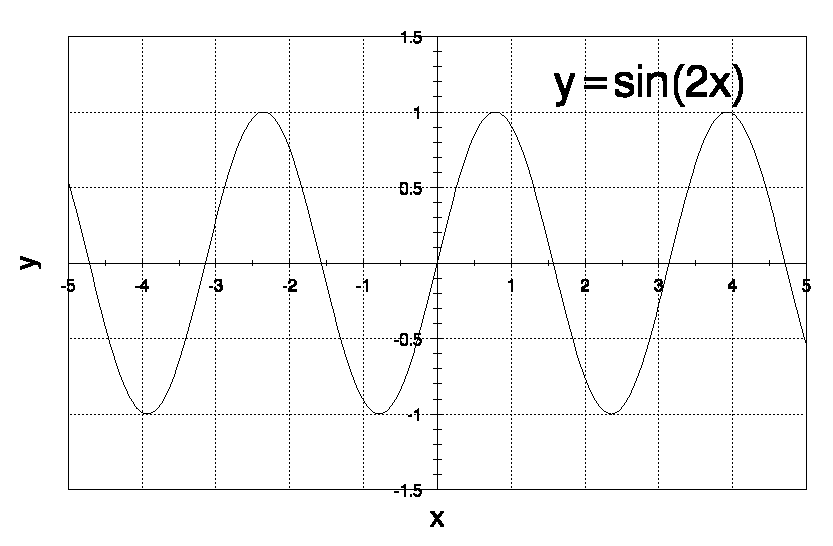
\includegraphics[width=\linewidth]{Figures/plot2.eps}
%%    \caption{This is a graph of the above equation, where the circular
%%      frequency is taken as $\omega = 2$.\label{fig1} Note: \emph{if
%%        you need to cite a source (of e.g.~a figure) in the caption,
%%        include the FULL CITATION, e.g.~} Source: Montezuma
%%      Publishing, San Diego State University Dissertation and Thesis
%%      Manual: Policies, Procedures and Format, Spring
%%      2010. \cite[\S 4.10.4 Figures]{DTM2010spring}}
%%  \end{minipage}
%%\end{figure}
%
%%\begin{figure}[ht]
%%  \centering
%%  \begin{minipage}{4.5in}
%%    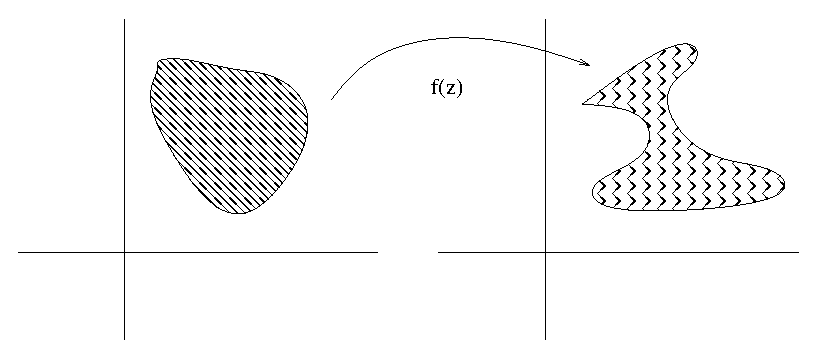
\includegraphics[width=\linewidth]{Figures/mapping.eps}
%%    \caption{Mapping $f(x)$ from the complex plane to itself. \label{fig:graph}}
%%  \end{minipage}
%%\end{figure}
%
%
%When you have a collection of figures and large figures, you may want
%to delay insertion of them until the end of the chapter. At the end of
%this chapter we are including a full page figure (Fig.~\ref{fullfig})
%to demonstrate this \LaTeX\ command. Note that if you cannot obtain
%postscript figures or are having too much trouble using the technique
%described above, then you can use the \verb+\vspace+ command to
%provide an empty space in the manuscript, then use the old-fashioned
%technique of taping in your figure and photocopying it.
%
%% 
%% If you have oversize full page figures, the following
%% might come in handy
%% 
%% \figurecoversheet{\label{figure:oversize} Caption goes here}
%
%
%\section{Tables}
%
%The Department of Mathematical Sciences does not have specific
%requirements on the exact layout of a table. However, the tables
%should be easily readable and properly labeled according to the
%regulations in the SDSU Thesis Manual. In this section we want to
%demonstrate how \LaTeX\ handles tables. More complicated examples can
%be found in Lamport's book \cite{LAM,LAM2}. We begin with a small table,
%given by Table \ref{tab1} which inserts nicely into the text.  Note
%that the same centering trick as was employed for figures is done here
%and we set the width of the \texttt{minipage} environment to 1.9
%inches.
%% 
%
%\begin{table}[hbt]
%  \centering
%  \begin{minipage}{1.9in}
%    \caption{A Small Table for Listing Some Parameters Used in Some
%      Numerical Procedure\label{tab1}. LONG CAPTION--- The Department
%      of Mathematical Sciences does not have specific requirements on
%      the exact layout of a table. However, the tables should be
%      easily readable and properly labeled according to the
%      regulations in the SDSU Thesis Manual.}
%    \begin{tabular}{|c||c|c|c|c||}    \hline
%      Trial &	a  &  b & c & $\omega$ \\ \hline \hline
%      1 & 5 & 10  & 15 & $\pi$ \\ \hline
%      2 & 10 & 20  & 15 & $2\pi$ \\ \hline
%    \end{tabular}
%  \end{minipage}
%\end{table}
%% 
%
%The\marginpar{\small\textbf{\textit{Style note}}} manual however
%allows for the caption to be a little wider if the table is really
%small and so we can use a wider \texttt{minipage} and then center the
%table inside there.  See for example Table \ref{wtab} where we used
%width of 3.5 inches.
%% 
%\begin{table}[hbt]
%  \centering
%  \begin{minipage}{3.5in}
%    \centering
%    \caption{Another Small Table for Listing Some Parameters Used in a
%      Numerical Procedure\label{wtab}.}
%    \begin{tabular}{|c||c|c|c|c||}    \hline
%      Trial &	a  &  b & c & $\omega$ \\ \hline \hline
%      1 & 5 & 10  & 15 & $\pi$ \\ \hline
%      2 & 10 & 20  & 15 & $2\pi$ \\ \hline
%    \end{tabular}
%  \end{minipage}
%\end{table}
%
%Note that you can use the \texttt{center} environment instead of
%\texttt{$\backslash$centering} but that might add a little bit of
%unwanted whitespace.  With \texttt{$\backslash$centering} on the other
%hand, you might have to put braces around the text you wish to center
%and sometimes need to add a \texttt{$\backslash$par}.  If you use it
%inside a \texttt{minipage}, \texttt{table} or \texttt{figure}
%environment, you don't have to really worry about that.  Note however
%that without the use of \texttt{minipage} you cannot center the
%caption as it automatically left aligns itself to conform with the
%thesis manual.
%
%Tables can also be left aligned see for example Table \ref{ltab}.
%Here we don't use the \texttt{minipage} environment, but we must then
%add linebreaks so that the table caption does not go wider then the
%table itself.  We need to add then two titles, one for the list of
%tables and one for the caption here.  The former will not have line
%breaks and the latter will.
%% 
%\begin{table}[hbt]
%  \caption[
%  Another Such Table but Left Aligned]{
%    Another Such\\Table but Left Aligned\label{ltab}}
%  \begin{tabular}{|c||c|c|c|c||}    \hline
%    Trial &	a  &  b & c & $\omega$ \\ \hline \hline
%    1 & 5 & 10  & 15 & $\pi$ \\ \hline
%    2 & 10 & 20  & 15 & $2\pi$ \\ \hline
%  \end{tabular}
%\end{table}
%
%Sometimes a table might not fit onto a single page, in this case you
%must not use the \texttt{table} environment, but instead the
%\texttt{longtable} environment.  Do note that \texttt{longtable}
%automatically centers so you need not worry about that.  See Table
%\ref{totallyrandom} for some absolutely random numbers.  To use
%\texttt{longtable} environment you must include the \texttt{longtable}
%package in your preamble. \textbf{see the note in \texttt{thesis.tex}
%  on how to fix the longtable entries in the ``List of Tables'' if
%  they are incorrect.}
%
%\begin{longtable}{|l|l|l|}
%  % You may need to modify the \LTcapwidth if the title wraps too early, or
%  % if it makes your table too large
%  % \LTcapwidth=6in
%  \caption{A Table of Some Totally Random Numbers} \label{totallyrandom} \\
%
%  % Here are our column headings
%  \hline
%  \multicolumn{1}{|l|}{\textbf{First}} &
%  \multicolumn{1}{l|}{\textbf{Second}} &
%  \multicolumn{1}{l|}{\textbf{Third}} \\
%  \hline \hline
%  \endfirsthead
%
%  % Here is the caption on other pages
%  \caption*{\tablename\ \thetable{} (Continued)} \\
%  \hline \multicolumn{1}{|l|}{\textbf{First}} &
%  \multicolumn{1}{l|}{\textbf{Second}} &
%  \multicolumn{1}{l|}{\textbf{Third}} \\ \hline \hline
%  \endhead
%
%  \multicolumn{3}{r}{\textbf{(table continues)}}
%  \endfoot
%
%  \hline
%  \endlastfoot
%
%  $16883.20050 \times 64.19591$ & $23174^{2905}$ & $(5112,5468,27117)$ \\ \hline
%  $7216.3398 \times 12239.16770$ & $19961^{9127}$ & $(16136,21997,26051)$ \\ \hline
%  $15977.29588 \times 5732.19698$ & $14995^{26728}$ & $(28634,14278,17183)$ \\ \hline
%  $24699.2338 \times 8803.18474$ & $19221^{28853}$ & $(18539,6044,19259)$ \\ \hline
%  $21444.11156 \times 24727.15793$ & $18372^{28126}$ & $(28032,2375,15319)$ \\ \hline
%  $4391.18511 \times 4548.30442$ & $1720^{1369}$ & $(3406,21419,16364)$ \\ \hline
%  $30135.17285 \times 30643.14550$ & $9216^{213}$ & $(23353,27690,19435)$ \\ \hline
%  $19438.13461 \times 25479.5929$ & $2137^{3868}$ & $(30657,17930,22240)$ \\ \hline
%  $26015.13194 \times 24615.8566$ & $17585^{10358}$ & $(13114,15259,12079)$ \\ \hline
%  $14483.18666 \times 730.30848$ & $16033^{18015}$ & $(28723,30583,27231)$ \\ \hline
%  $28936.21168 \times 22153.15603$ & $7838^{2847}$ & $(8315,13767,4984)$ \\ \hline$12183.11656 \times 22915.1655$ & $4903^{3341}$ & $(26271,13469,20927)$ \\ \hline
%  $3861.26584 \times 3418.15940$ & $8299^{22084}$ & $(16670,6379,5349)$ \\ \hline
%  $1917.2334 \times 3164.29148$ & $31271^{24332}$ & $(18534,14106,32170)$ \\ \hline
%  $21381.22421 \times 13170.26365$ & $1836^{24826}$ & $(16512,3492,29730)$ \\ \hline
%  $19854.29763 \times 10431.8013$ & $856^{4247}$ & $(11431,16797,12547)$ \\ \hline$748.699 \times 18926.6097$ & $2617^{21261}$ & $(9262,31765,19764)$ \\ \hline
%  $826.17531 \times 1102.229$ & $6144^{23524}$ & $(13399,32510,25360)$ \\ \hline
%  $5457.16254 \times 28852.2419$ & $3340^{25847}$ & $(12851,11353,26704)$ \\ \hline
%  $17098.22785 \times 10733.29645$ & $23533^{11432}$ & $(15804,29630,14049)$ \\ \hline
%  $4297.6124 \times 13047.24061$ & $6951^{30578}$ & $(25163,7180,3955)$ \\ \hline
%  $15919.20579 \times 3697.8512$ & $26036^{19951}$ & $(4596,28456,23292)$ \\ \hline
%  $30444.8539 \times 1877.24380$ & $25637^{24662}$ & $(2345,22515,15427)$ \\ \hline
%  $13777.5551 \times 12290.27827$ & $9848^{18414}$ & $(8106,1141,25365)$ \\ \hline$5916.26304 \times 32545.9871$ & $9456^{20356}$ & $(13568,17968,13625)$ \\ \hline
%  $752.22564 \times 9313.24044$ & $20240^{17852}$ & $(25921,11852,10721)$ \\ \hline
%  $17816.14197 \times 468.475$ & $27975^{6019}$ & $(12765,23034,15867)$ \\ \hline
%  $31180.31140 \times 17008.23777$ & $4288^{10545}$ & $(23555,14160,20001)$ \\ \hline
%  $11143.27728 \times 5201.24768$ & $28480^{27765}$ & $(1313,19756,15238)$ \\ \hline
%  $19165.12910 \times 27090.29887$ & $30726^{8520}$ & $(30355,31201,3727)$ \\ \hline
%  $3607.11199 \times 26761.19474$ & $9611^{25133}$ & $(3715,620,29421)$ \\ \hline
%  $14260.24175 \times 10813.1493$ & $2551^{5774}$ & $(6694,27319,1486)$ \\ \hline
%  $1691.28633 \times 21243.16929$ & $15030^{1385}$ & $(11252,12149,32111)$ \\ \hline
%  $19772.9737 \times 30544.23499$ & $13344^{8975}$ & $(17492,50,18586)$ \\ \hline
%  $9857.3765 \times 19207.6510$ & $18025^{10614}$ & $(17324,19518,13165)$
%
%\end{longtable}
%
%
%
%
%A larger table, given by Table \ref{tab2} and reproduced from another
%document, then you may need to allow an entire page for the
%table. This is done by typing the command
%\verb+\begin{table}[p]+. This test example is included in the
%minipage environment to show how a footnote\footnote{We also need to
%  see how a regular footnote appears in the text, so one was inserted
%  here. Multiple lines are easily handled by \LaTeX.}  can be added to
%a table.  Several problems have been noted before on how \LaTeX\
%handles the location of the table in the text.
%\begin{table}[p]
%  \centering
%  \begin{minipage}{3.7in}
%    \caption{Computations for Products of the \emph{RRN} Genes at Different
%      Growth Rates\label{tab2}}
%    \begin{tabular}{|c||c|c|c|c|c||}	 \hline
%      $\tau$(min)  &  100  &	60 & 40 & 30 & 24 \\ \hline \hline
%      $C$ period & 67 & 50  & 45 & 43 & 42 \\ \hline
%      $D$ period & 30 & 27  & 25 & 24 & 23 \\ \hline
%      $V_0$ & 0.437 & 0.577 & 0.815 & 1.15 & 1.63 \\ \hline
%      $\bar c$\footnote{$\times 1000\ {\rm ribosomes}/\mu{\rm m}^3$.}
%      & 11.1 & 16.8 & 22.1 & 28.1 & 31.4 \\ \hline
%      $\bar c_{85}$\footnote{$\times 1000\ {\rm ribosomes}/\mu{\rm m}^3$,
%        representing the average concentration of the product of the
%        \emph{rrn} gene located at $85'$.} & 1.73 & 2.68 & 3.65 & 4.81
%      & 5.57 \\ \hline 
%      $\bar c_{57}$\footnote{$\times 1000\ {\rm ribosomes}/\mu{\rm m}^3$,
%        representing the average concentration of the product of the \emph{rrn} gene
%        located at $57'$.} & 1.36 & 1.98 & 2.43 & 2.87 & 2.96 \\ \hline
%      $\bar c_{85}({\scriptstyle\times 100})/\bar c$\footnote{Percentage of
%        $\bar c$ produced by the \emph{rrn} gene located at $85'$.} & 15.6 & 15.9 &
%      16.5 & 17.1 & 17.7 \\ \hline
%      $\bar c_{57}({\scriptstyle\times 100})/\bar c$\footnote{Percentage of
%        $\bar c$ produced by the \emph{rrn} gene located at $57'$.} & 12.3 & 11.8 &
%      11.0 & 10.2 & 9.44 \\ \hline
%      $\bar c_{85}/\bar c_{57}$ & 1.27 & 1.35 & 1.50 & 1.68 & 1.88 \\ \hline
%      $r$\footnote{Initiations/min/gene.} & 3.75 & 10.27
%      & 22.56 & 38.42 & 56.98 \\ \hline
%      $c_{max}$\footnote{$\times 1000\ {\rm ribosomes}/\mu{\rm m}^3$, representing
%        the maximum concentration during the cell cycle.} & 11.28 & 17.04
%      & 22.33 & 28.36 & 31.77 \\ \hline
%      $c_{max}/c_{min}$\footnote{Ratio of maximum to minimum concentration
%        during the cell cycle.} & 1.041 & 1.036 & 1.027 & 1.024 & 1.026 \\ \hline
%    \end{tabular}
%  \end{minipage}
%\end{table}
%
%%\begin{figure}[p]
%%  \centering
%%  \begin{minipage}{4.5in}
%%    \includegraphics[width=\linewidth]{Figures/somb.eps}
%%    \includegraphics[width=\linewidth]{Figures/cos.eps}
%%    \caption{The top graph is the function $z = \sin(r)/r$, while
%%      the bottom surface is the function $z = \cos(r)$. \label{fullfig}}
%%  \end{minipage}
%%\end{figure}
%
%
%
%\section{Potential Pitfalls}
%
%\subsection{Tables and Figures}
%
%There is a conflict between the \verb+\usepackage{subfig}+,
%\verb+\usepackage{caption}+ and the \verb+sdsu-thesis.cls+ class
%specification.  The long table captions show up correctly (bold and
%left aligned with table).  Use \verb+\usepackage{subfigure}+ instead
%and all captions, as well as the list of tables page show up ok.
%
%If you insist on \verb+\usepackage{subfig}+, make sure to
%\textbf{first} issue the command
%\verb+\usepackage[bf,labelsep=period,textfont=bf]{caption}+ where the
%first "\verb+bf+" makes the labels "Figure n" bold;
%\verb+labelsep=period+ says "use '.' instead of ':'; and
%\verb+textfont=bf+ makes the caption text bold.  This may solve your
%subfig problems.
%
%
%Table captions (``table titles'' \cite{DTM2010spring}) go
%ABOVE\marginpar{\small\textbf{\textit{Style note}}} the table, must be
%in \emph{headline style} where ``all major words are capitalized,''
%and there is no period at the end of the caption; in figure captions
%only the first word is capitalized, and there is a period at the
%end. --- \textbf{THE STYLE DOES NOT CURRENTLY ENFORCE THIS, \emph{YOU}
%  HAVE TO DO IT MANUALLY.}
%
%Charts, graphs, diagrams, maps, photographs, and other graphic
%illustrations should all be labeled as \emph{Figures} \cite[\S4.6.9,
%and \S4.10.4]{DTM2010spring}.  Figure captions are capitalized
%sentence style in the text; therefore, the List of Figures entries
%should be in sentence style.
%
%All tables and figures must be referenced in text \emph{prior} to
%their appearance. Those references should be by number.
%
%
%
%\subsubsection{Centered Tables Figures}
%\label{sec::centered:tab:fig}
%
%It is not as simple as adding \verb+\centering+ into the figure or
%table environment as that will center the caption on the page rather
%then left align it with the left edge of the figure or table.  So the
%way to solve this is to figure out the width of the figure or table
%and add it in a minipage and center that.  For example if our table is
%2 inches wide when typeset, then we could do
%\begin{verbatim}
%\begin{table}[ht]
%  \centering
%  \begin{minipage}{2in}
%    \caption{Caption goes here}
%    ... here is your table ...
%  \end{minipage}
%\end{table}
%\end{verbatim}
%
%
%
%\subsection{Margins}
%
%It is believed that the \verb+sdsu-thesis.cls+ template complies with
%the SDSU thesis manual: 1.25 inch left, 1 inch top, bottom and right.
%But your \emph{printout} may not give the right measurement, if your
%printer/printer-driver scales the document.  You may have to turn off
%scaling and/or tweak the settings in the \verb+sdsu-thesis.cls+ file.
%
%Someone said: \emph{``Some laser printers don't do the margins correctly, for
%example my printer shifts the page a bit.  You can correct this with
%the} \verb+\hoffset+ \emph{and} \verb+\voffset+ \emph{lengths as:}\\
%\hspace*{2em}\verb+\hoffset -0.0625in+\\
%\hspace*{2em}\verb+\voffset  0.15625in+''
%
%
%\subsection{Bad Pagebreaks}
%
%Sometimes LaTeX does not do exactly what you want with respect to
%pagebreaks.  To solve this you can manually add a \verb+\pagebreak+
%command where it should break, or you could add
%\verb+\enlargethispage{12pt}+ to make a page slightly larger if
%needed; though I'm not sure how the thesis reviewer will look on such
%transgressions, so do that at own risk.
%
%Bad pagebreaks in the table of contents (or list of tables/figures):
%If you get a bad pagebreak in a table of contents you can force a
%pagebreak by: \verb+\addtocontents{toc}{\protect\pagebreak}+ you add
%this at the point in your document that corresponds to that place in
%the table of contents.  For list of tables and list of figures,
%replace `toc' in the line above with `lot' or `lof.'
%
%
%\subsection{Bad Linebreaks}
%
%Bad linebreaks in chapter, section (subsection, etc...), or
%table/figure caption titles: This classfile tries to make all titles
%conform to the requirements of the thesis manual, but it is possible
%that it gets things wrong and  to add linebreaks (the
%\verb+\\+ command) yourself.  However, the table of contents title
%should not have any linebreaks.  The way you do it is to add an
%optional argument to \verb+\chapter+, \verb+\section+,
%\verb+\caption+ as in:\\
%\hspace*{2em}\textbf{$\backslash$chapter[Title for Table of
%  Contents]\{Title With$\backslash$$\backslash$Linebreaks\}}\\
%Note that for \verb+\caption+'s in figures and tables you might have
%to do this whenever you have a small figure or table as the
%table/figure environment cannot make the caption only as long as the
%figure since it doesn't know how large the figure is until it typesets
%everything.  See example above and more examples in the long-example
%directory.  You can also solve the \verb+\caption+ issue with minipage
%in the same way we do centering, see
%section~\ref{sec::centered:tab:fig}.
%
%
%
%\subsection{Vertical Space}
%
%This classfile tries to make all the vertical space as required, but
%sometimes you may need to modify what it does, or you just need to
%insert some vertical space.  You use the \verb+\vspace+ and
%\verb+\vspace*+ commands (see \LaTeX\ manual).  You can use positive
%or negative length there and \verb+\vspace*+ makes sure the space appears
%even if there is a pagebreak in between.  For example to add 2 inches
%of space you can add \verb+\vspace{2in}+.
%
%
%\subsection[Non-Bold Math in the TOC: $x=2\pi/e$]{Bold Math in the Thesis:  $\mathbf{x=\pi}$}
%
%Math in section titles need to be \textbf{bold}, but cannot be bold in
%the Table of Contents.

\chapter{RESULTS AND DISCUSSION} \label{chapter:Results}
In this chapter results are presented for several simulated conditions.

\begin{enumerate}
	\item Nominal vs. dispersed parameters
	\item Atmosphere vs. vacuum
	\item Static initial conditions vs. dynamic ignition timing
\end{enumerate}

The first condition, the effect of dispersion, is of interest on the topic of robustness. A closed-loop guidance law implementation is intended to ensure satisfaction of the problem constraints in practical conditions with uncertainty of state and performance limitations. A guidance system without periodic state feedback, i.e. an open-loop implementation, would be expected to quickly lose accuracy and ultimately fail in real application. Due to the criticality of safety in the intended mission, it is vital to show that this strategy performs well in nominal as well as dispersed conditions and to give a sense for the uncertainty in its performance.

The second condition is of particular interest because, as is clear in Section \ref{sec:guidancelaw}, neither E-Guidance nor the Gravity Turn approach take into account atmospheric effects and, at least in the case of the Apollo missions, have not been flown in the context of atmospheric landing. It is important to verify that the strategy can satisfy mission goals and still perform well in atmosphere, and the comparison with vacuum conditions serves both as a control and a fuel requirement baseline. 

The third condition is the subject of this study. Whether dynamic ignition timing can reliably provide propellant efficiency improvement while maintaining safety and practicality is the topic of interest.

\subsection{Vacuum Performance}
Presented first are nominal results for the non-atmospheric condition. The starting conditions are listed in Table \ref{tab:IC}. These conditions represent points along a ballistic trajectory which misses the landing site by a small angle at altitude

\subsection{Atmospheric Performance} \label{sec:results_atmosphere}

\subsection{Discussion}
Here we interpret results, discussing agreement and disagreement with expected performance as well as sources of error and mitigation methods.

%Middle chapter.  Here we put the middle things, that is, things that
%are in the middle and not in the beginning or in the end.  Here we
%also test all the section, subsection, and other headings.
%
%\textbf{Note\marginpar{\small\textbf{\textit{Style note}}} that
%  CHAPTER TITLES need to be in ALL CAPS --- YOU have enter the chapter
%  titles in ALL CAPS!!!}
%
%\section{A Section}
%
%Some section text.  Note that there should ALWAYS be some text in
%between two sectioning levels; a \verb+\section+ directly followed by
%a \verb+\subsection+ will not go through the review.
%
%\subsection{A Subsection With a Very Long Title To See How That Will
%  Look When Printed}
%
%Some subsection text.
%
%\subsubsection{A Subsubsection}
%
%Some subsubsection text.
%
%\subsubsubsection{A Subsubsubsection}
%
%Some subsubsubsection text.  If you are using this, you are
%\sout{probably} over-organizing things.
%
%\paragraph{A Paragraph.}
%
%Some paragraph text.  You never really get this deep --- don't be
%ridiculous.

\chapter{CONCLUSIONS AND FUTURE WORK}



\chapter{REFERENCING}

%Below a list of references are provided in the acceptable format for
%Master's thesis submission. References are to be numbered and should
%appear either alphabetically or in the order of appearance in the
%text.  (\LaTeX\ does the former for the student.) For students using
%\LaTeX\ these are obtained using the plain style with {\sc
%Bib}\TeX. The Department of Mathematics and Statistics will accept
%either the plain style or the SIAM style. (For the SIAM style, get a
%copy of the SIAM.BST file from your graduate adviser or the
%Mathematical Sciences computer system.) There are references for
%journal \verb+article+s \cite{ART}, \verb+book+s and \verb+booklet+s
%\cite{BOK,BKL}, \verb+inbook+s, \verb+incollection+s, and
%\verb+inproceedings+
%\cite{INC,INB,INP}. \emph{Note\marginpar{\small\textbf{\textit{Style
%note}}} that when you have more than one citation in a single bracket
%they must be in increasing numerical order!}  Other sources may be
%\verb+proceedings+ \cite{PRO}, technical reports (\verb+techreport+)
%\cite{TEC}, theses (\verb+mastersthesis+, or \verb+PhDthesis+)
%\cite{MTH}, or \verb+unpublished+ material \cite{UNP}.  This should
%provide a fairly comprehensive list for any material that the student
%may encounter.  For additional assistance, see the graduate adviser in
%your area of concentration. \LaTeX\ source codes are available for
%copying.
%
%If you cite a website \cite{Wikipedia} and you can't find the year on
%the website, you should put "n.d." (not dated) at the end. (this is
%true for other reference also.) It must also has the word "accessed"
%and the month and year you access the website.  You can change how
%things with no author(s) are sorted in the bibliography by supplying a
%\verb+key+ entry (see \verb+thbib.bib+), \emph{e.g.} this news release
%\cite{EPA-2010-09-07} will be sorted under ``U,'' the leading letter
%of the publishing agency (as preferred by the thesis publisher).
%
%This \cite{PatentExample} is an example of a patent.
%\textbf{\textit{Notice:}} how the \texttt{month} and \texttt{year}
%fields in \texttt{thbib.bib} have been abused to force the ``correct''
%format.
